\section{Quantifying Baryon Redistribution}
\label{sec:feedbackmetrics}

Feedback is a complex process that impacts a wide range of
baryonic observables, from the galaxy stellar mass function, to galaxy sizes,
to the density profiles of galaxies \citep[e.g.][]{BenitezLlambay2018}. It is
interesting, therefore, to develop tools to study the global effects of
feedback directly, as a complement to the many indirect constraints
obtainable from comparing to astrophysical observables. Here we describe the
tools we will use to examine the redistribution of baryons via feedback.

The kinetic feedback scheme used in \simba{} for both star formation and AGN
feedback makes it straightforward to identify the gas elements that have been
directly impacted by feedback. However, these gas elements will then go on to
entrain and deposit energy into other gas elements as they travel. This makes
it challenging to fully capture the impact of feedback solely from particle
tagging. Another option to assess feedback is to run simulations with
specific feedback modules turned on and off. However, this is inconsistent
with the tuning procedure that virtually every simulation suite performs in
order to constrain the many parameters in the sub-grid model. For instance,
modern models are typically calibrated to the $z=0$ Stellar Mass Function
(SMF), which will of course change should some feedback mechanism be missing
(and hence should be re-calibrated). It is thus important to realize that, if
without some feedback module a simulation fails to match data, this does not
definitively prove that the feedback module is necessary to produce realistic
galaxies, since it could potentially be that the simulation could be
recalibrated to match data in some other way. In our case, we run the \nojet{}
and non-radiative variants in order to explore how baryon redistribution is
sensitive to these feedback modules, but we do not attempt to recalibrate
these to data, and merely use them in order to investigate the impact of this
input physics within the context of the \simba{} model.

\subsection{The Spread Metric}

\begin{figure}
    \centering
    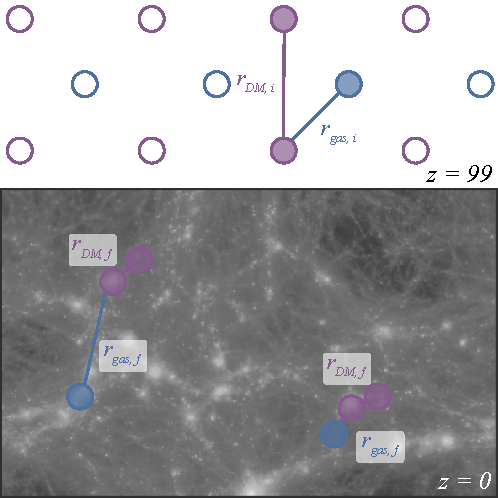
\includegraphics[width=\columnwidth]{figures/kspafig_small.pdf}
    \vspace{-0.5cm}
    \caption{The matching procedure between initial and final conditions
    illustrated. The top panel shows the $z=99$ initial conditions, where
    every particle finds its nearest dark matter neighbour. The bottom
    panel shows the distances between those particles at $z=0$. For the
    fiducial result, each particle actually finds the three nearest 
    neighbours in the initial conditions and takes the median at $z=0$
    of these distances (see text for explanation) but this is omitted
    in this simple picture for brevity.}
    \vspace{-0.5cm}
    \label{fig:kspafigsmall}
\end{figure}

Our approach to quantifying the large-scale impact of feedback is to develop
a simple and robust metric that directly captures the displacement of the gas
owing to feedback. This `spread' metric, illustrated in Figure
\ref{fig:kspafigsmall}, works as follows:

\begin{enumerate} 
	\item For every particle $i$ in the initial conditions, find the nearest
          $n$ dark matter neighbours $j$ (with $n=3$ for the fiducial result).
	\item In the final conditions, match all remaining baryonic particles
	      with their initial conditions progenitor (in this case, stars are
	      matched with their gas progenitor).
	\item In the final conditions, find the distance $r_{ij}$, i.e. the
	      distance between the particle and its original neighbours. The spread metric for
	      this particle is then given as the \emph{median} of these $n$
	      distances.
\end{enumerate}

\begin{figure}
    \centering
    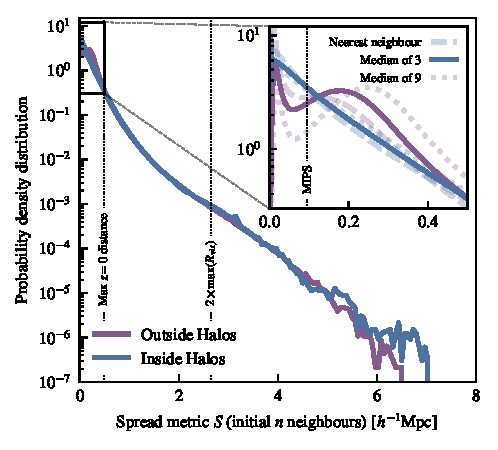
\includegraphics{figures/s50j7kAHF/dark_matter_distance_figure_s50j7k_AHF}
    \vspace{-0.5cm}
    \caption{The distribution of final-state distances from the spread metric
    for dark matter in the full \simba{} model run. This distribution is
    relatively unchanged by the choice of sub-grid model, and the effects of
    the back-reaction of baryonic physics on dark matter is out of the scope
    of this work. The distribution is split between particles that lie within
    halos and those that lie outside, with this being an approximately even
    split at $z=0$. Lines are over-plotted to show the maximal distance
    between any two dark matter particles at $z=0$, approximately
    $0.5\hmpc{}$, and twice the maximal virial radius of any halo in the box,
    which is approximately $1.3\hmpc{}$. The inset figure shows the inner
    $0.5\hmpc{}$ of the distribution, and has a line over-plotted for the
    mean inter-particle separation in the initial conditions (MIPS) of
    approximately $0.1\hmpc$. The fainter lines show how the low-spread
    distribution changes when taking the average over a number of initial
    nearest neighbours; dashed gives the metric with no median (i.e. only one
    nearest neighbour), and the dotted line shows the case for a median over
    9 neighbours. }
    \vspace{-0.5cm}
    \label{fig:dmonlyspread}
\end{figure}

The `spread' metric is presented first for dark matter in Figure
\ref{fig:dmonlyspread}. The simplest metric here clearly is simply to use the
nearest neighbour in the initial conditions, rather than the median over $n$
initial neighbours. The choice of $n=3$ was made primarily to ensure that the
dark matter results were robust when comparing matter inside and outside of
halos. For a given dark matter particle pairing, a large distance between two
neighbours would be `double counted' for the case where one neighbour makes
it into a halo and one remains outside, contributing the large distances to
both bins. Choosing $n=3$ enables the median result to represent the distance
to a real particle, and removes the problem of double counting for the
nearest neighbour. The overall distributions of distances were not changed
much by this choice, however larger choices for $n$ increase the contrast in
the dark matter images in Figure \ref{fig:bigdistanceimage}, with more
substructure picked up in the low-spread particles, and show more diffuse
structure in the high-spread particles.

\subsection{Baryon Spreading in \simba{}}

Figure \ref{fig:distbaryon} shows how the distribution of spread distances
for the gas particles is significantly different to that for the dark matter.
Gas particles are able to be spread to much larger distances, up to $12\hmpc{}$,
compared to the $7\hmpc{}$ that dark matter can reach. We also see that even
halo gas is spread more than the dark matter, when explicitly selecting for this
component.

Another interesting selection to make is the gas that originated in
lagrangian regions (i.e. next to dark matter that will reside in halos at
$z=0$). With the baryon fraction of halos being typically less than $50\%$ of
the cosmic value, we should expect that a lot of this gas is lost over time,
with this possibly being spread out to larger distances. This gas may also be
expelled from the halos in high energy events, either through stellar winds
or AGN feedback. In \simba{}, we see that this gas is spread systematically
further, with there being approximately a factor of two more particles at
spreads larger than $\sim 4 \hmpc{}$ than an unbiased selection would
suggest.

\begin{figure}
    \centering
    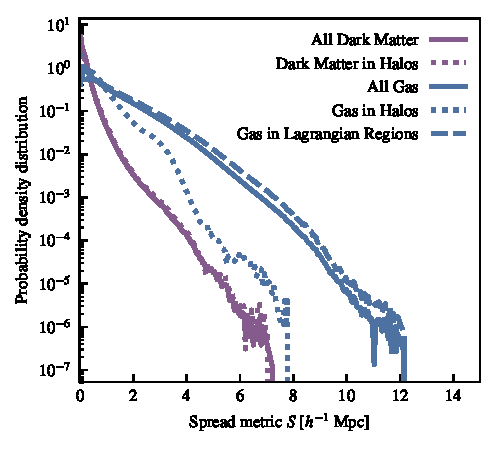
\includegraphics{figures/s50j7kAHF/distance_plot_split_by_component+AHF.pdf}
    \vspace{-0.5cm}
    \caption{The distance metric histogram, now including gaseous matter.
    Note how, compared to the dark matter, the distributions for gas inside
    halos and outside halos are significantly different, with gas that
    originated in lagrangian regions being preferentially moved to larger
    distances than gas on average. Note that only 10\% of the gas in the
    entire simulation is in halos at $z=0$. Gas can be blown out to
    $12\hmpc{}$, approximately 10 times the virial radius of the largest halo
    in the box.}
    \vspace{-0.5cm}
    \label{fig:distbaryon}
\end{figure}

\begin{figure*}
    \centering
    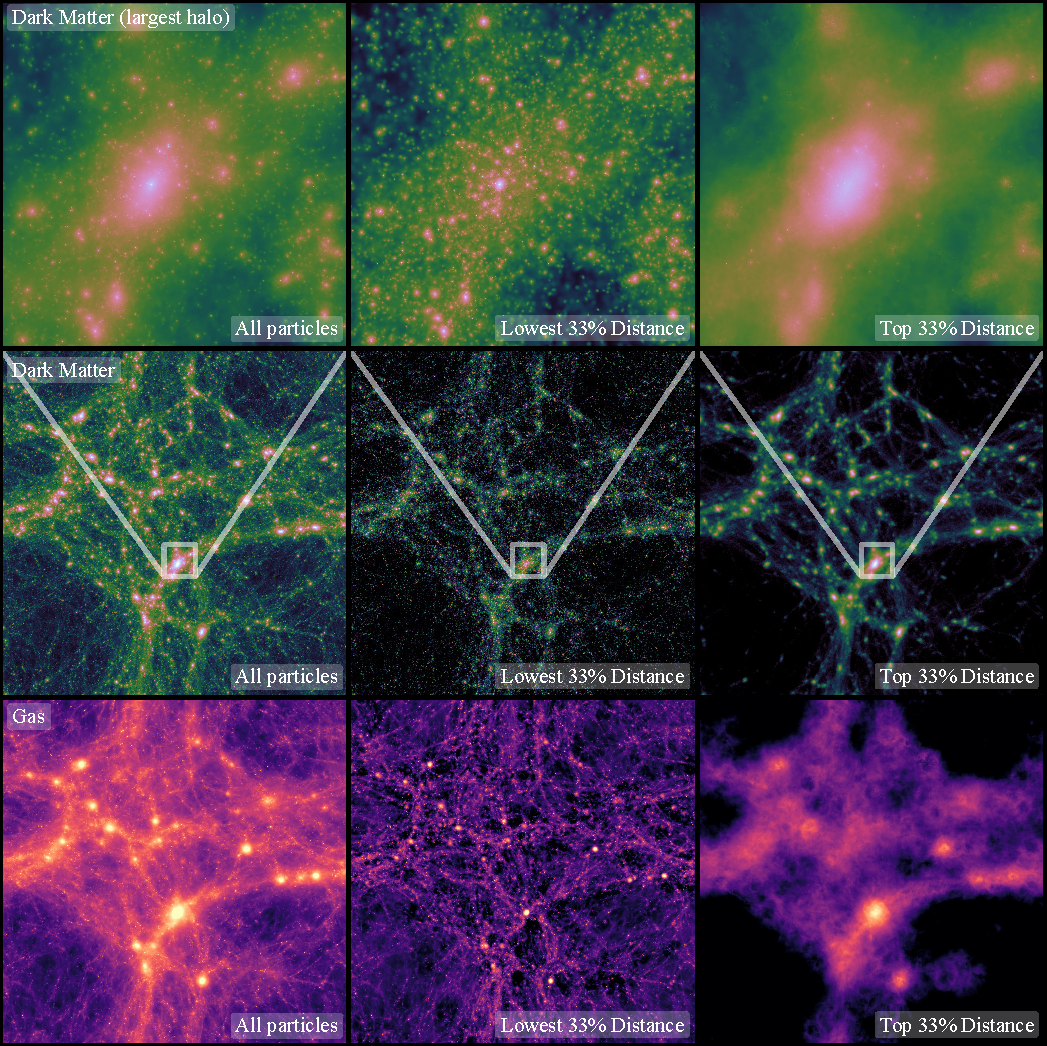
\includegraphics[width=\textwidth]{figures/distance_figures_3.pdf}
    \caption{The three rows show the following selections of particles (from
    top to bottom): the dark matter present in the largest halo, and
    surrounding it (this is a $4.5\hmpc{}$ cube centred around the halo
    centre, which has a virial radius of approximately $1.3\hmpc{}$); all
    dark matter particles in the box; and all gas particles present in the
    box. All images are shown in the final state of the simulation at
    redshift $z=0$. Each column then shows (from left to right): all
    particles that are in the volume; the particles that have spread the
    least, selecting the first 33\% from the histogram figures; and the
    particles that have spread the 33\% most. For the dark matter, these cuts
    correspond to particles that have travelled less than $0.1\hmpc{}$, and
    greater than $0.25\hmpc{}$ respectively. For the gas, these numbers
    increase to $0.45\hmpc{}$ and $1.25\hmpc{}$ respectively due to the
    larger spread that these particles experience. Each image has smoothing
    lengths generated to encompass $32$ nearest neighbours, as is used in the
    \simba{} simulations, and smoothing lengths are kept consistent across
    columns; i.e. they are not re-smoothed. All images in a given row also
    use the exact same (logarithmic) normalisation and colour map to enable
    comparisons. Note how even with this extremely conservative cut there is
    a significant difference between the images, with sub-structure picked
    out by the low-distance cut and large-scale structure for the
    large-distance cut.}
    \vspace{1cm}
    \label{fig:bigdistanceimage}
\end{figure*}

These significantly different spread distributions should correspond to
significantly different real-space distributions. In the below we define
`low-spread' particles as those in the lower tertile (33\%) of the
distribution, and `high-spread' particles as those that are in highest
tertile of the distribution.

A visualisation of the low- and high-spread particles is show in Figure
\ref{fig:bigdistanceimage} for both dark matter and gas, for the fiducial
\simba{} model. By making (generous) cuts in the distance distribution, we
are able to show that the low-spread particles correspond to substructure,
with the high-spread particles contribution being the larger-scale, more
diffuse, CGM and IGM.

Considering first the dark matter in the largest halo, the top row of panels,
we see that the very small-scale substructure of the halo, including the central
density peak itself, is picked up by the low-spread particles. The
diffuse component of the dark matter tha fills the space between these individual
subhalos is identified in the high-spread particles, with only a small
amount of residual sub-structure remaining. These trends are also clear in the
view of the whole box shown in the second row, with the majority of the dark matter
filaments being shown in the high-spread panel. It is interesting to note that
a large amount of the structure in the voids is not present in either of these
panels, with it being captured by the medium-spread particles with spread
metric values $0.1\hmpc{} < r_{ij} < 0.25 \hmpc{}$.

The final row shows the gas particles, cut with the same proportions (however
note that this corresponds to different absolute values of the spread
metric). The low-spread gas particles trace the cores of galaxies and their
disks, along with some residual filamentary structure. Of particular note is
the high-spread gas particles, which trace the large bubbles that the strong
AGN jets in the \simba{} model produce, allowing for gas that is entrained by
these feedback events to be systematically identified.

\begin{figure*}
    \centering
    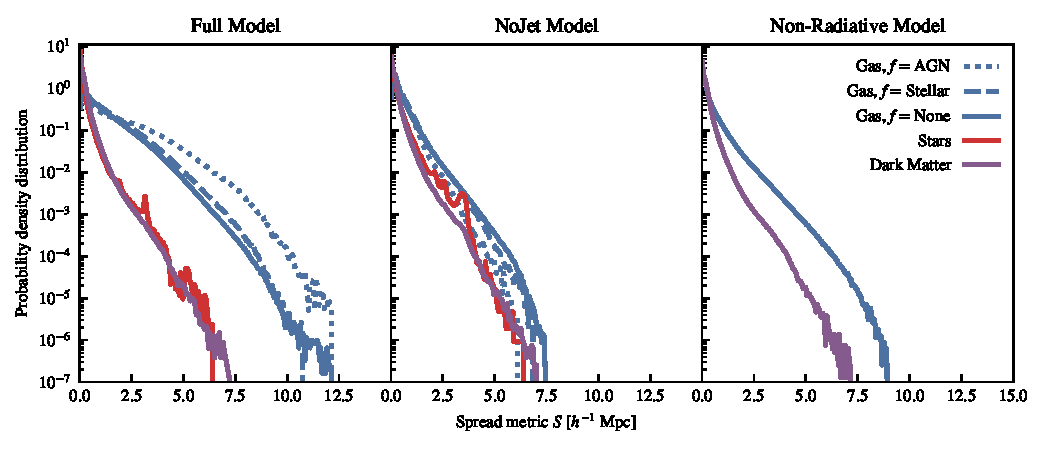
\includegraphics[width=\textwidth]{figures/neighbour_analysis_feedback_histogram_combined.pdf}
    \vspace{-0.7cm}
    \caption{The (normalised) distribution of distances for all particles
    $i$ to the nearest neighbour $j$ in the initial conditions, split by
    particle type. This is shown for the $z=0$ particle distribution in the
    reference model (left), \nojet{} model (center), and a non-radiative run
    (right). Splitting the particles by those that have been involved in
    feedback events in this figure shows that the further out a particle has
    been blown the more likely it is to have been directly involved in a
    feedback event for the reference model. Also note the vertical $0.5-1$
    dex offset for gas compared to dark matter even in the \nojet{} run.
    }\label{fig:feedbackdistance}
\end{figure*}

In Figure \ref{fig:feedbackdistance}, we show different models in an
attempt to better characterise the effects of different pieces of the
\simba{} sub-grid model.

The left panel, showing the full \simba{} model, also splits the 
gas component into particles that have been affected by different
types of feedback. Here, AGN feedback takes precedence over stellar
feedback, such that if a particle has been affected by both it is only
classified as being part of the $f=$AGN group. We see that the particles
that have directly interacted with the AGN are spread to significantly 
larger distances, with a vertical 0.5-1 dex offset for a given spread
metric bin at large values. Particles that have been directly kicked by
stellar feedback also have systematically higher spread metric values,
albeit with a much smaller offset. This implies that particles are being
spread to these large distances by the feedback events.

The left panel also now includes the stellar matter, which shows a very tight
correspondence to the dark matter distribution, despite having formed out of
gas particles. This is expected by redshift $z=0$, as since cosmic noon at
around $z=2$ where star formation peaks, there has been many Gyrs for these
particles to virialise and relax back into equilibrium with the dark matter.
It would be unexpected for a star particle to form from a gas particle with a
high spread value, as these must have been separated dynamically from their
closest dark matter neighbour, requiring some kind of energy injection into
the gas phase. This would heat the particle, likely to a high temperature,
preventing the particle from having long enough to cool by $z=0$ to a
temperature low enough to form a star.

The specific effect of the high-energy AGN jets is shown in the second panel
on Figure \ref{fig:feedbackdistance}. This \nojet{} run still includes some
thermal feedback from the AGN, with only the jets removed. With this
(seemingly small) change, the spread metric is transformed completely,
showing a much tighter correspondence between the dark matter, gas, and
stars. Thanks to strong cooling flows, particles that have been directly
heated by feedback (those in the densest regions) actually now show a lower
spread metric than an average particle, with dark matter and gas in these
dense regions unable to dynamically separate from each other.

This result is surprising given that less than $0.4\%$ of gas particles in
the simulation have ever interacted directly with the AGN jets; this has been
enough to completely separate the majority of the gas from the dark matter
dynamically. Such a high degree of separation points to huge amounts of gas
being entrained by these powerful jets. It is not simply the case that higher
mass ($M_H > 10^{11} \msolar{}$) halos are quenched internally reducing their
star formation rate; the energetics and dynamics of the CGM and IGM are
significantly altered, as is already seen by the more complex interaction
between the turn-off of the galaxy stellar mass function (GSMF) and the power
of the AGN jets in many studies.

The final contrast to highlight is the difference between the \nojet{} and
non-radiative model. The non-radiative model shows increased distance between
gas particles and their associated dark matter neighbour compared to the
\nojet{} run; this due to the lack of cooling preventing particles that lie
in small halos from remaining as tightly bound. It also highlights how
difficult it is to drive gas into the centers of structures without cooling.
The collisionless dark matter can continue to fall in to bound structures,
with the gas being prevented due to strong accretion shocks. This allows for
a very different kind of separation than what we conjectured above about the
full physics models that include cooling.

\begin{figure}
    \centering
    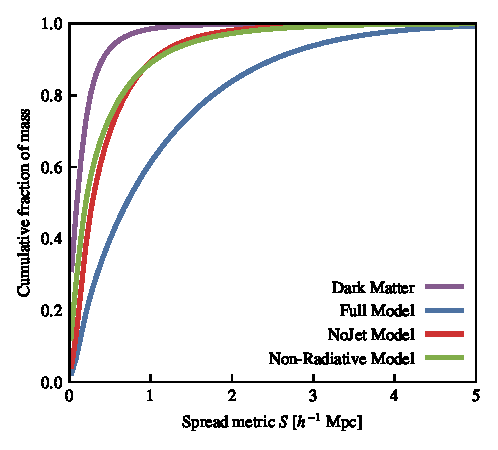
\includegraphics{figures/cumulative_histogram_comparison.pdf}
    \vspace{-0.7cm}
    \caption{Cumulative version of Fig. \ref{fig:feedbackdistance} that
    shows the gas distribution for the three models alongside the dark
    matter from the full model.}
    \label{fig:cumulativehistogram}
\end{figure}

In Fig. \ref{fig:cumulativehistogram} we show the cumulative version of Fig.
\ref{fig:feedbackdistance} to better show the amounts of mass that are spread
to large distances. The full model constrains about 90\% of the mass within
around $3\hmpc{}$, with a slow tail off ending with nearly all of the mass
being constrained to be spread less than $5\hmpc{}$.

These results show that gaseous and stellar matter can be transferred out to
significantly further (by $z=0$) than is assumed by typical zoom-in
simulation suites. For example, the Latte \citep{Wetzel2016} suite uses an
exclusion region for high resolution particles of around $1.5 \hmpc{}$.
Whilst they do not find contamination (possibly due to isolation criteria) of
low-resolution particles into the high-resolution region, the above metrics
suggest that perhaps this is a more numerical, rather than physical, effect;
low resolution particles are not present due to a lack of sub-grid physics in
the unrefined region.
